\documentclass[12pt]{article}
\usepackage{common}
\usepackage{amsmath}
\usepackage{setspace}
\usepackage{graphicx}
\usepackage{tikz}
\tikzset{> = latex, every picture/.style={line width=0.7pt}}

\pdfpagewidth 8.5in
\pdfpageheight 11in 

\setlength\topmargin{0in}
\setlength\headheight{0in}
\setlength\headsep{0in}
\setlength\textheight{9in}
\setlength\textwidth{5.5in}
\setlength\oddsidemargin{.5in}
\setlength\evensidemargin{.5in}
\setlength\parindent{0.25in}
\setlength\parskip{0in}

\newboolean{solutionCopy}
\setboolean{solutionCopy}{true} % Toggle between solution copy and distro

\ifthenelse{\boolean{solutionCopy}}{
  \includeversion{solution}
}{
  \excludeversion{solution}
}

\begin{document}

\title{CS 181: Markov Decision Processes and Reinforcement Learning}
\author{Yamini Bansal, Sam Melton, Mark Goldstein}
\date{Week of April 16, 2018}
\maketitle

\section{Markov Decision Processes}

A Markov Decision Process (MDP) is a framework for modeling an
agent's actions in the world. It consists of:
\begin{enumerate}
\item A set of states $S$
\item A set of actions $A$
\item A reward function $r: S \times A \rightarrow \reals$
\item A transition model $p(s'| s, a)$, $\forall s,s' \in S, a \in A$.
\end{enumerate}
A \textit{policy} $\pi$ is a mapping from states to actions, i.e. $\pi: S \to A$. 

\subsection{Finite time horizon MDP}

In the finite horizon setting, a policy may vary with the number
of time periods remaining. $\pi_{(t)}$ denotes the
policy with $t$ time steps
to go. $T$ is the decision horizon. The value of a policy
with $t$ time steps to go
 is defined inductively
to be:
\begin{align} 
V^\pi_{(t)}(s) = \begin{cases}
r(s, \pi_{(1)}(s))
 & \text{if } t = 1 \\ 
r(s, \pi_{(t)}(s)) + \sum_{s' \in S} p(s' | s, \pi_{(t)}(s)) V^\pi_{(t-1)}(s') & \text{o.w.}\end{cases}
\end{align}

The process of computing these values inductively,
working from the end of the horizon to the present, 
is called
\textit{value iteration}.  
If we instead look forward in time, we
 are  computing the expected
value of the policy
%
%
\begin{align} V^\pi(s) = \mathbb{E}_{s_1,\ldots,s_T}\left[\sum_{t=1}^T r(s_t, \pi_{(T+1-t)}(s_t))\right] \end{align}
by induction, where $s_1 := s$. $V^\pi(s)$ is the MDP value function.

In an MDP, the general goal is to find an optimal policy  by maximizing the expected reward under the policy, i.e. maximizing the value function. This is the \emph{planning problem}.

% \vspace{1pc}

% \noindent {\bf Exercise 1: Value Iteration}

% \vspace{.5pc}

% \noindent \fbox{\parbox{\linewidth}{%
% Say an MDP has reward function $r$ with $r(s, a) > 0, \forall s \in S, a \in A$. If you run value iteration, what is the largest $k$ for which $V_k(s)$ is zero? }}

% \vspace{.5pc}

% \begin{solution}
% \noindent Solution: $k=0$. $V_0(s) = 0$ for all states $s$. Since $V_1(s) = \max_{a \in A}\{ r(s, a) \} $ and all rewards are positive, all $V_k(s) >0$ when $k > 0$.
% \end{solution}

% \vspace{.5pc}

\subsection{Infinite Horizon MDP}

\paragraph{Policy Evaluation}

We can also send $T \to \infty$, i.e. have an infinite time horizon. In that case, we need a discount factor $0 < \gamma < 1$, and we want to compute the value function
\begin{align}
V^\pi(s) = \mathbb{E}_{s_1,s_2,\ldots}\left[\sum_{t=1}^\infty \gamma^{t-1} r(s_t, \pi(s_t))\right]\end{align}
where $s_1 := s$, and the $\gamma$ factor ensures convergence (assuming bounded rewards). In this setting, we only worry about stationary policies that don't vary with time.
This is the \emph{policy evaluation} problem; for any given policy $\pi$, we can find $V^\pi(s)$ by solving the system of linear equations
\begin{align}V^\pi(s) = r(s, \pi(s)) + \gamma \sum_{s' \in S} p(s' | s, \pi(s)) V^\pi(s') \label{eq:bellman_policy_eval} \end{align}
These capture consistency about the value function. To solve this system, we can use Gaussian elimination, or simply iterate until convergence as in the finite horizon case.

\paragraph{Value Iteration}

Suppose we have an optimal policy $\pi^*$. This satisfies the following set of equations known as the \emph{Bellman equations}:
\begin{align}V^*(s) = \max_{a \in A} \left[r(s,a) + \gamma \sum_{s' \in S} p(s' | s, a) V^*(s')\right] \end{align}
where $V^* \triangleq V^{\pi^*}$. Assuming we know $V^*$, we can read off the optimal policy
by setting 
\begin{align}
\pi^{*}(s) = \argmax_{a \in A}\left[r(s, a) + \gamma \sum_{s' \in S} p(s'|s, a) V^\ast(s') \right] \label{eq:vi_opt_policy}
\end{align}

\noindent In order to find $V^*$, we can use \emph{value iteration}:

\begin{itemize}
    \item Initialize: $V(s) = 0$ for all states $s$.
    \item Update step (Bellman operator):
    \begin{align}
    V'(s) = \max_{a\in A}\left[r(s,a) + \gamma\sum_{s'\in S}p(s'|s,a)V(s')\right], \text{  } \forall s
    \end{align}
    \item $V \leftarrow V'$
\end{itemize}
% \begin{align} 
% V^*_{(t)}(s) = \begin{cases}0 & \text{if } t = 0 \\ 
% \max_{a \in A} \left[r(s, a) + \gamma \sum_{s' \in S} p(s' | s, a)(s)) V^*_{(t-1)}(s')\right] & \text{o.w.}\end{cases}
% \end{align}
where we iterate until convergence of $V$, which is guaranteed. With our converged $V$, we can then find $\pi^*$ as in Equation \ref{eq:vi_opt_policy}.

\vspace{.5pc}

\paragraph{Policy Iteration}

\noindent Another approach to planning is called \textit{policy iteration}. To do policy iteration, we evaluate a proposed policy $\pi$ by finding $V^\pi$ as in Equation \ref{eq:bellman_policy_eval}. This is Evaluation step (E step).
Then, we do a policy improvement step (I step) by the equation
\begin{equation}
\pi'(s) \gets \argmax_{a \in A} \left[ r(s,a) + \gamma \sum_{s' \in S} p(s'|s,a)V^\pi(s') \right], \quad \forall s
\end{equation}
We repeat the E and I steps until the policy $\pi$ converges (stops changing).

Note that policy iteration takes more computation per iteration, but tends to converge faster in practice.


\section{Reinforcement Learning}

In the general reinforcement learning setting, we don't have access to the transition distribution $p(s'|s,a)$ or the reward function $r(s,a)$ --- information about these only come to us through the outcome of the environment. 
This problem is hard because some states can lead to high rewards, but we don't know which ones; even if we did, we don't know how to get there!

To deal with this, in lecture, we discussed \textit{model-based} and \textit{model-free} reinforcement learning. 


\subsection{Model-based Learning}

For model-based learning, we estimate the missing world models: $r(s, a)$ and $p(s'|s, a)$, and then utilize planning (value or policy iteration) to develop a policy $\pi$.


\vspace{1pc}

\noindent {\bf Exercise 1: Model Building}

\vspace{.5pc}

\noindent \fbox{\parbox{\linewidth}{%
Question: How would we do this in practice? What is the downside of this approach?
 }}

\vspace{.5pc}

\begin{solution}
\noindent {\bf Solution:} One approach is to do a number of random walks. At each state, take a random action. Track the rewards you get in the states you transition to. You can use these to estimate the probability distributions for the transitions, and the average reward for each state-action pair. Downside: If there are many states and/or actions, the transition model $p(s'|s,a)$ becomes huge. May be hard to get a good estimate of the true model. Also, the goal is not to learn the transition model - it is to learn an optimal policy (so we may be do unnecessary work).
\end{solution}

\vspace{.5pc}




\subsection{Model-Free Learning}

In model-free learning, we are no longer interested in learning the transition function and reward function. Instead, we are looking to directly infer the optimal policy from samples of the world --- that is, given that we are in state $s$, we want to know the best action $a = \pi^*(s)$ to take.

To do this, we use an alternate formulation of the Bellman equations, which states that for an optimal policy $\pi^*$,
\begin{align}
Q^*(s,a) = r(s,a) + \gamma\sum_{s' \in S}p(s' | s, a)\max_{a' \in A}[Q^*(s', a')], \text{  } \forall s,a \label{eq:q_bellman}
\end{align}

Then, once we have $Q^*$, we note that
\begin{align}
\pi^*(s) = \argmax_aQ^*(s, a)
\end{align}

The question then becomes how we can find the Q values that satisfy the Bellman equations as written in Equation~\ref{eq:q_bellman}. To do this, we parameterize $Q(s,a; \boldw)$ with parameters $\boldw$, where $w_{s,a} = Q(s,a;\boldw)$ is a table of estimated Q values. We define a loss function which we want to minimize:

\begin{align}
\mcL(\boldw) = \frac{1}{2}\mathbb{E}_{s,a}\left( Q(s,a; \boldw) - [r(s,a) + \gamma\sum_{s'}p(s'|s, a)\max_{a'}Q(s', a'; \boldw)
]\right)^2
\end{align}

We can optimize this via stochastic gradient descent. In order to get samples to perform gradient descent on, the idea is to approximate the loss by sampling $s,a$, giving a single gradient descent step
\begin{align}\frac{\partial \mcL}{\partial w_{s,a}} = Q(s,a;\boldw) - [r(s,a) + \gamma \sum_{s'}p(s'|s, a)\max_{a'}Q(s', a'; \boldw)]\end{align}
If we can obtain a sample for the next state $s'$ and the reward $r$ from the environment, we can approximate this as
\begin{align}\frac{\partial \mcL}{\partial w_{s,a}} \approx Q(s,a;\boldw) - [r + \gamma \max_{a'}Q(s', a'; \boldw)]\end{align}

This is the term that we will use to update our estimates for $Q$:
\begin{align}
w_{s,a} \leftarrow w_{s,a} - \eta\frac{\partial \mcL}{\partial w_{s,a}}
\end{align}
where $\eta>0$ is the learning rate.

\subsection{Exploration vs. Exploitation}

How do we actually obtain the above samples to approximate the loss? The key issue here is \emph{exploration vs. exploitation}.

In an exploitative approach, when we are in state $s$, we can simply take action $a = \argmax_{a \in A} Q(s,a;\boldw)$ based on our current estimate of the Q-function. However, if our estimate of the Q-function is bad, we might never find the true best action this way.

In an explorative approach, we might pick an action at random --- one method is $\epsilon$-greedy, where we take $\argmax_{a \in A} Q(s,a;\boldw)$ with probability $1-\epsilon$, and pick $a \in A$ uniformly at random with probability $\epsilon$ (for some $\epsilon>0$).

We want to balance these two --- exploitation lets us arrive at the optimal policy faster, but exploration is necessary to properly understand the state space. In practice, $\epsilon$-greedy is a good policy for minimizing $\mcL$.

\subsection{On-Policy vs. Off-Policy}

Suppose we now have a policy $\pi$ that balances exploration and exploitation (e.g. $\epsilon$-greedy). To satisfy the Bellman equations for $Q^*(s,a)$, 
the policy would need to take the optimal actions in all future steps. Obviously, this won't always be true if we are exploring.

Therefore, there are multiple ways to write the gradient estimate $\partial \mcL / \partial w_{s,a}$. These are about how to learn, not about which explore/exploit policy to follow. One approach is \emph{on-policy}:
\begin{equation}
\frac{\partial \mcL}{\partial w_{s,a}} \approx Q(s,a;\boldw) - [r + \gamma Q(s', \pi(s'); \boldw)]
\end{equation}
where $r$ and $s'$ are given to us from the environment.

This is known as the SARSA update (State-Action-Reward-State-Action), since we look ahead to get the action $\pi(s')$. Since we follow $\pi$ in choosing this action, this gradient method is on-policy. In practice this converges faster, but we lose the guarantee of satisfying the Bellman equations (and thus may not converge to the optimal
policy).

Another approach is \emph{off-policy}:
\begin{equation}
\frac{\partial \mcL}{\partial w_{s,a}} \approx Q(s,a;\boldw) - [r + \gamma \max_{a' \in A} Q(s', a'; \boldw)]
\end{equation}
This is know as the Q-learning update. This uses State-Action-Reward-State from
the environment. Since we take a max over actions $a'$ for the gradient update, we are going `off-policy.' This takes longer to converge, but our update is consistent with the Bellman equations.

To summarize, no matter what our gradient estimate is, we make the gradient update
\begin{equation}
w_{s,a} \gets w_{s,a} - \eta \frac{\partial\mcL}{\partial w_{s,a}}
\end{equation}
For the case of Q-learning, this can be written as
\begin{align}
w_{s,a} &\gets w_{s,a} - \eta \left( w_{s,a} - [r + \gamma \max_{a' \in A} Q(s', a'; \boldw)] \right) \\
&= (1-\eta) w_{s,a} + \eta  [r + \gamma \max_{a' \in A} Q(s', a'; \boldw)]
\end{align}
Essentially, we are interpolating the old value of $w_{s,a}$ with an estimate of the future value.\\

\noindent Similarly, for SARSA, the update is
\begin{align}
w_{s,a} &\gets w_{s,a} - \eta \left( w_{s,a} - [r + \gamma  Q(s', \pi(s'); \boldw)] \right) \\
&= (1-\eta) w_{s,a} + \eta  [r + \gamma  Q(s', \pi(s'); \boldw)]
\end{align}

\section{Exercises}

(Sutton \& Barto 2012) Consider an MDP on the following grid:

\begin{center}
\begin{tikzpicture}
\draw[step=1cm] (-2,-2) grid (1,1);
\node at (-0.5,+0.5) {A};
\node at (-0.5,-1.5) {B};
\end{tikzpicture}
\end{center}

At each square, we can go left, right, up, or down. Normally we get a reward of 0 from moving, but if we attempt to move off the grid, we get a reward of $-1$ and stay where we are. Also, if we move onto square A, we get a reward of 10 and are teleported to square B.

Suppose our actions also fail with probability 0.5, i.e. with probability 0.5 we stay on the current square.

Suppose our MDP is infinite horizon, and take $\gamma = 0.9$ to be the discount factor.

\vspace{.5pc}

\noindent \fbox{\parbox{\linewidth}{%
\textbf{Defining the MDP} Identify the states $S$, actions $A$, rewards, and transition probabilities $p(s'|s,a)$ in this problem.
}}

\vspace{.5pc}

\begin{solution}
There are 9 states, one for each square of the grid, which we will denote as $(i,j)$ for $i=0,1,2$ (rows) and $j=0,1,2$ (columns), where $(0,0)$ is the top left corner. There are 4 actions (one for each direction), call them L,R,U,D.

We will define $r(s,a)$ for a state-action pair as the expected reward from taking action $a$ in state $s$; for example, $r((0,0), R) = 0.5 \times 0 + 0.5 \times 10 = 5$.\footnote{An earlier version of this handout treated the reward as if the robot could control its environment, but its actuator is noisy. Thus, we should adopt $r(s,a)$ to be defined as the expected reward for taking action
  $a$ in state $s$.}
%
%  , we defined $r(s,a)$ as the reward you get from taking action $a$ in state $s$ ASSUMING it's successful. While this is a legitimate definition of the reward function, it makes less sense in a real world setting, where you expect to fail half the time.)

The probabilities of transition between any two valid states are all 0.5, and the probabilities of remaining at any state are all 0.5 (except for moving off the edge of the board, where the probability is 1 of staying). In addition, a
successful transition into state $A$ results in the agent being in state $B$ (teleportation!).
%transition from $(0,0)$ to $(2,1)$ has probability 0.5 (teleportation from A to B).
\end{solution}

\vspace{.5pc}
\noindent \fbox{\parbox{\linewidth}{%
\textbf{Policy Evaluation} Suppose $\pi$ is the policy where we always choose to go right. Write the equations to find the values $V^\pi(s)$.
}}

\vspace{.5pc}


\begin{solution}
\noindent {\bf Solution:} Recall the policy
evaluation equations
$$V^\pi(s) = r(s,\pi(s)) + \gamma \sum_{s' \in S} p(s'|s, \pi(s)) V^\pi(s')$$

We have
\begin{align*}
    V^\pi((0,0)) &= 5 + (0.9)(0.5 \times V^\pi((0,0)) + 0.5 \times V^\pi((2,1)) \\
    V^\pi((0,1)) &= 0 + (0.9)(0.5 \times V^\pi((0,1)) + 0.5 \times V^\pi((0,2)) \\
    V^\pi((0,2)) &= -0.5 + (0.9) V^\pi((0,2))  \\
    V^\pi((1,0)) &= 0 + (0.9)(0.5 \times V^\pi((1,0)) + 0.5 \times V^\pi((1,1)) \\
    V^\pi((1,1)) &= 0 + (0.9)(0.5 \times V^\pi((1,1)) + 0.5 \times V^\pi((1,2)) \\
    V^\pi((1,2)) &= -0.5 + (0.9) V^\pi((1,2))  \\
    V^\pi((2,0)) &= 0 + (0.9)(0.5 \times V^\pi((2,0)) + 0.5 \times V^\pi((2,1)) \\
    V^\pi((2,1)) &= 0 + (0.9)(0.5 \times V^\pi((2,1)) + 0.5 \times V^\pi((2,2)) \\
    V^\pi((2,2)) &= -0.5 + (0.9) V^\pi((2,2)) \\
\end{align*}
We can compactly write this in matrix form as follows:
$$\boldV = \boldr + \gamma \boldT \boldV$$
where
\begin{align*}
    \boldV = [&V^\pi((0,0)), V^\pi((0,1)), V^\pi((0,2)), \\
&V^\pi((1,0)), V^\pi((1,1)), V^\pi((1,2)), \\
&V^\pi((2,0)), V^\pi((2,1)), V^\pi((2,2))]^\top
\end{align*}
$$\boldr = [5, 0, -0.5, 0, 0,-0.5, 0, 0, -0.5]^\top $$
$$\boldT = \begin{bmatrix}
0.5 & 0 & 0 & 0 & 0 & 0 & 0 & 0.5 & 0 \\
0 & 0.5 & 0.5 & 0 & 0 & 0 & 0 & 0 & 0 \\
0 & 0 & 1 & 0 & 0 & 0 & 0 & 0 & 0 \\
0 & 0 & 0 & 0.5 & 0.5 & 0 & 0 & 0 & 0 \\
0 & 0 & 0 & 0 & 0.5 & 0.5 & 0 & 0 & 0 \\
0 & 0 & 0 & 0 & 0 & 1 & 0 & 0 & 0 \\
0 & 0 & 0 & 0 & 0 & 0 & 0.5 & 0.5 & 0 \\
0 & 0 & 0 & 0 & 0 & 0 & 0 & 0.5 & 0.5 \\
0 & 0 & 0 & 0 & 0 & 0 & 0 & 0 & 1 \\
\end{bmatrix}$$
Note that the policy affects $\boldr$ and $\boldT$. This linear system can be solved using standard methods (e.g. Gaussian elimination). We find that (approximately)
$$\boldV = [ 5.7, -4.1, -5, -3.4, -4.1, -5, -3.4, -4.1, -5]$$
\end{solution}

\vspace{.5pc}

\noindent \fbox{\parbox{\linewidth}{%
\textbf{Value Iteration} Write the second iteration of value iteration, i.e. starting by initializing $V(s) = \max_{a \in A} r(s,a)$.
}}

\vspace{.5pc}


\begin{solution}
\noindent {\bf Solution:} Note that initially we have
\begin{align*}
    V((0,0)) = 5, \, V((0,1)) = 0, \, V((0,2)) = 5 \\
    V((1,0)) = 0, \, V((1,1)) = 5, \, V((1,2)) = 0 \\
    V((2,0)) = 0, \, V((2,1)) = 0, \, V((2,2)) = 0 \\
\end{align*}

For state $(0,0)$ we have the update:
\begin{align*}
    V'((0,0)) &= \max [-0.5 + (0.9) \times V((0,0)) ,\\
            &            -0.5 + (0.9) \times V((0,0)) , \\
            &            5 + (0.9) (0.5 \times V((0,0)) + 0.5 \times V((2,1))) , \\
            &            0 + (0.9) (0.5 \times V((0,0)) + 0.5 \times V((1,0))) ] \\
            &= \max [-0.5 + (0.9)(5), \\
            &-0.5 + (0.9)(5), \\
            &5 + (0.9)(0.5 \times 5 + 0.5 \times 0), \\
            &0 + (0.9)(0.5 \times 5 + 0.5 \times 0)] \\
            &= 7.25
\end{align*}
by taking the max over each of the four directions (left, up, right, down in that order). You can verify that the following hold for the remaining states:
\begin{align*}
    V'((0,1)) = 2.25, \, V'((0,2)) = 7.25 \\
    V'((1,0)) = 2.25, \, V'((1,1)) = 7.25, \, V'((1,2)) = 2.25 \\
    V'((2,0)) = 0, \, V'((2,1)) = 2.25, \, V'((2,2)) = 0
\end{align*}
\end{solution}

\vspace{.5pc}

\noindent \fbox{\parbox{\linewidth}{%
\textbf{Policy Iteration} Write the first iteration of policy iteration, starting with $V^\pi(s) = 0$ for all $s$. (We could also initialize a policy, and do the Evaluation
step to get started.)
}}

\vspace{.5pc}


\begin{solution}
\noindent {\bf Solution:} Let's first do the I step (policy Improvement) to find
the new policy $\pi'$. For $(0,0)$, considering that we assume
$V^\pi(s)$ under the current policy, we have
$$\pi'((0,0)) = \argmax_{a \in A} [ -0.5, -0.5, 5, 0] = \text{R}$$
For other states, we get
\begin{align*}
    \pi'((0,0)) = \text{R}, \,\pi'((0,1)) = \text{R}, \, \pi'((0,2)) = \text{L} \\
    \pi'((1,0)) = \text{R}, \, \pi'((1,1)) = \text{U}, \, \pi'((1,2)) = \text{D} \\
    \pi'((2,0)) = \text{R}, \, \pi'((2,1)) = \text{R}, \, \pi'((2,2)) = \text{U}
\end{align*}
breaking ties arbitrarily.

Next we do the E step (Evaluation). This is policy evaluation, and we can write our equation as $\boldV = \boldr + \gamma \boldT \boldV$, where
% $\boldV$ is the same as before, but now we have
%
based on the current policy $\pi'$ we have
%
$$\boldr = [5, 0, 5, 0, 5, 0, 0, 0, 0]^\top$$
$$\boldT = \begin{bmatrix}
0.5 & 0 & 0 & 0 & 0 & 0 & 0 & 0.5 & 0 \\
0 & 0.5 & 0.5 & 0 & 0 & 0 & 0 & 0 & 0 \\
0 & 0 & 0.5 & 0 & 0 & 0.5 & 0 & 0 & 0 \\
0 & 0 & 0 & 0.5 & 0.5 & 0 & 0 & 0 & 0 \\
0 & 0 & 0 & 0 & 0.5 & 0.5 & 0 & 0 & 0 \\
0 & 0 & 0 & 0 & 0 & 0.5 & 0 & 0 & 0.5 \\
0 & 0 & 0 & 0 & 0 & 0 & 0.5 & 0.5 & 0 \\
0 & 0 & 0 & 0 & 0 & 0 & 0 & 0.5 & 0.5 \\
0 & 0 & 0 & 0 & 0 & 0.5 & 0 & 0 & 0.5 \\
\end{bmatrix}$$
Solving for $\boldV$, we find that
$$\boldV = [9.1, 7.5, 9.1, 7.5, 9.1, 0, 0, 0, 0]^\top$$
is the new estimate for $V^{\pi'}$.
\end{solution}

\vspace{.5pc}

\noindent \fbox{\parbox{\linewidth}{%
\textbf{Q-learning} Suppose we are in the reinforcement learning setting where we don't know the transition probabilities $p(s'|s,a)$ or the reward function.

Suppose we start at the top left square and follow an $\epsilon$-greedy policy. At the beginning, suppose $Q(s,a) = 0$ for all $s,a$, except we know that we shouldn't go off the grid, so that the values of $Q$ for the corresponding $s,a$ pairs are $-1$. Take learning rate $\eta = 0.1$.
}}

\vspace{.5pc}

For the first step, suppose our policy tells us to explore, and we end up going right as our action (which succeeds). Write the Q-learning update.
\medskip

\begin{solution}
  \noindent {\bf Solution:}  Now that we work with reinforcement learning, we can handle the effect of the noisy actuator on the reward directly. The realized reward for an action, that is used as feedback, will depend on the state, the action, and whether or not the action succeeds.

  Our environment gives us $r = 10$ for succeeding and $s' = (2,1)$ for the next state. For Q-learning, we get an update to $w_{s,a}$ for $s=(0,0), a=\text{R}$ with gradient
$$\frac{\partial \mcL}{\partial w_{s,a}} = 0 - (10 + (0.9) \max [0,-1,0,0] )= -10$$
The max is taken over actions in $s'=(2,1)$ (where we end up).

This gives update
$$Q((0,0), \text{R}) = w_{s,a} = 0 - (0.1)(-10) = 1$$
We can also write this update as
$$w_{s,a} = (0.9)(0) + (0.1)(10 + 0.9 \times \max[0,-1,0,0]) = 1$$

\end{solution}

\vspace{.5cm}
\bigskip

Now write the SARSA update, assuming that our policy gives us a second action telling us to explore and go down (which also succeeds).
\bigskip

\begin{solution}
\noindent {\bf Solution:} Because $Q((2,1), \text{D}) = -1$ as we would go off the grid, we have gradient
$$\frac{\partial \mcL}{\partial w_{s,a}} = 0 - (10 + (0.9) \cdot (-1)) = -9.1$$
This gives us a slightly different update than in Q-learning:
$$Q((0,0), \text{R}) = w_{s,a} = 0 - (0.1)(-9.1) = 0.91$$
We can also write this update as
$$w_{s,a} = (0.9)(0) + (0.1)(10 + 0.9 \times (-1)) = 0.91$$
\end{solution}

\end{document}
